% !TEX root = ../Rulebook.tex
\label{sec:Competition}

The competition is held in the form of so called tests.
A test requires a robot to perform various abilities, including navigation, manipulation, task planning and autonomous decision making.
Different kinds of tests each have their focus a current research field, e.g. picking moving objects or efficient task execution.

All tests require a robot to autonomously navigate the arena defined in \ref{sec:ArenaDesign} without causing a collision. Each team can enter the arena before actual competitions to create a map of the environment and test their robot. The OC will organize time slots for each team respecting the amount of teams and available slots. Usually there will be some setup days that can be used only for training.

\section{Time Schedule}

The actual competition currently includes a total of 7 tests.
These are spread across available competition days, with test having time buffers in between each other.
An example for the schedule can be found here: \url{https://atwork.robocup.org/rc2021/}.
As on site events have tighter schedules and additionally require teams to prepare everything for an unknown environment, there will usually only be two setup and four competition days, maybe even less.
Teams should prepare for something like fig. \ref{fig:example_schedule}. 

\begin{figure}[h!]
\centering
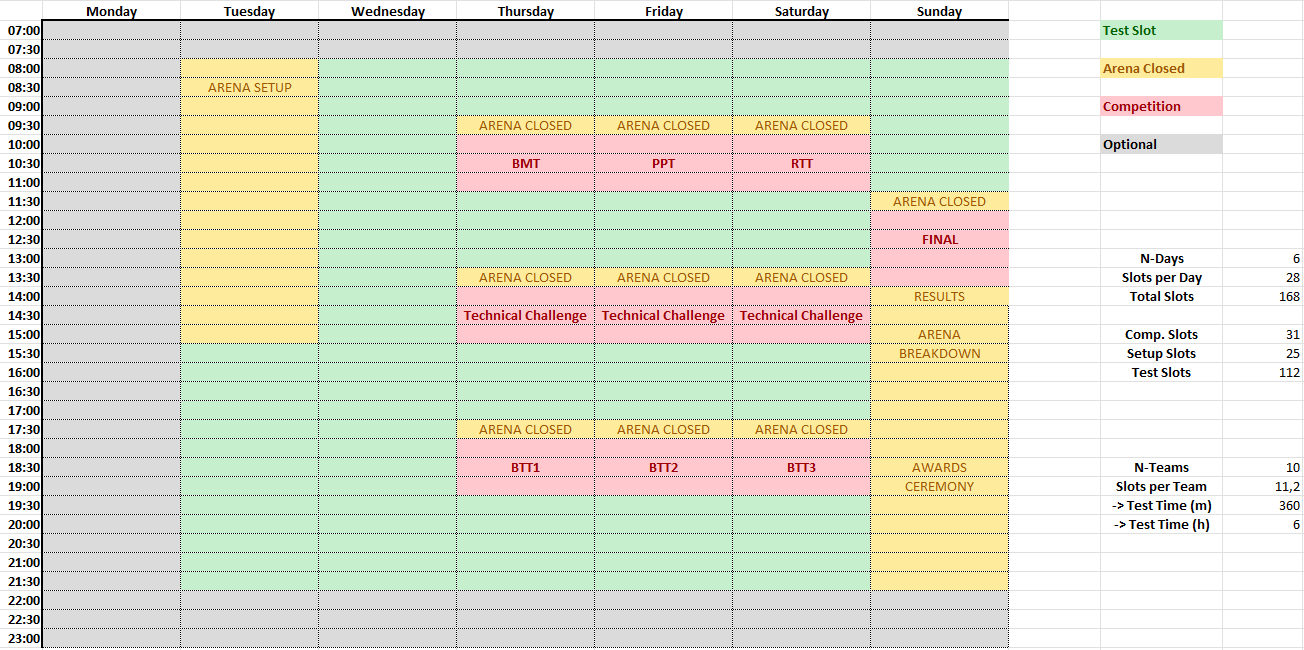
\includegraphics[width= 0.8\textwidth ]{./images/competition/example_schedule}
\caption{Example of a time schedule for a \RCAW competition.}
\label{fig:example_schedule}
\end{figure}

Team leaders are required to announce wether their team likes to participate in a test 1 hour prior to the start time to allow the OC to plan the schedule and create scoring sheets.

\section{Parc ferm\'e}

All participating teams must bring their performing robot to the parc ferm\'e 15 minutes before a test and leave them there during the whole timeslot of the test, except when they must perform.
Rules similar to motorsports apply: The robot must not be worked on or changed in any kind unless
serious damage must be repaired. This intends to encourage teams to watch other performances while still give teams the chance to remain in the competition. It is allowed to attach a charger to the robot.

The location of the parc ferm\'e will be towards the spectators for entertainment.
The robots may (are wished to) be turned on and ready to perform, enabling teams to set robot arm positions and illumination for the visitors. 

If the power management of a robot does not enable it to be turned on during the runs of other teams,
the specific team may power-on and boot their robot once the run of the previous team has ended.
They may not change or modify their robot in any way during this time (hardware and software).

\section{Test Procedure}

15 minutes before a competition slot the arena is set up for the upcoming test.
Therefore, the position of each static arena element is checked and objects are placed on active 
Service Areas.
The TC will decide where dynamic arena elements are placed 
and which orientation an object gets to create a starting setup for the test.
\lucas{TC or referees decide dynamic elements and only orientation?} 

Each team must nominate one person which acts as a referee during all tests.
The job of each ref is to ensure that the arena state before each performance is the same as the setup.
They also rate each performance. This ensures that the interests of every team are respected equally.

A performance slot for a team includes a preparation phase, the run phase and the end phase.

\textbf{Preparation Phase}

During the prep phase, teams are allowed to move their robot from the parc ferm\'e to the defined start pose in the arena either by hand or by carefully driving manually. They should prepare their robot for their run and can therefore remote access the robot and/or make minor changes.
It is explicitly forbidden to hardcode solutions for specific requirements of a test during this phase (e.g. drawing position of obstacles in the map). Also, if the robot passes and detects obstacles during this phase, they must be erased from the memory (e.g. clear costmap) unless they can be detected from the START location.

\textbf{Run Phase}

The run phase begins once the start time is up or when the teamleader announces that the team is ready. 
The task is then sent to the robot and from there on, the robot must act fully autonomously. It is forbidden to interact or control the robot in any human kind (keyboard/mouse actions, gestures, voice). The unplugging of a LAN cable to ensure that the task was send to the robot at bad WLAN connections is the only interaction with the robot that is allowed.
The run phase ends once the robot has stopped at the FINISH location of the arena, when the run time is up, when the teamleader says 'stop' or the robot caused a second Major Collision.

\textbf{End Phase}

In the resulting end phase the team is expected to move their robot back to parc ferm\'e.
Referees gather and discuss their performance rating afterwards.
Once they agree on the performing team's result, 
the teamleader is required to accept this score. 
Teams are allowed to make their case if they do not agree with the refs decision,
but cannot force changes and are expected to be understanding.
Special cases will be decided by the TC if the rulebook leaves room for interpretation.

Once the score has been accepted by a team,
the arena must be set up for the next run if necessary.
The prep time of the next team begins once the arena state is declared as ready by all refs.

TODO ADD TABLE 

\section{Skipping Tests}

If a team decides not to participate in a test during the official time slot, this test type may be repeated once during a following time slot. This should enable struggling teams to do the more simpler tests later in the competition. This option should only be used by teams if really necessary to keep the structure of the overall competition. Also, teams are only allowed to perform a test with a lower potential total score than the current test.

